\documentclass[12pt]{article}
\usepackage[spanish]{babel}
\usepackage{geometry}
\geometry{a4paper, margin=1in}
\usepackage{graphicx}
\usepackage{xcolor}
\usepackage{titlesec}
\usepackage{parskip}
\usepackage{multicol}
\usepackage{cite}
\usepackage{listings}
\usepackage{color}
\usepackage{amsmath}
\usepackage{enumitem}

\lstset{
  language=Python,
  basicstyle=\ttfamily\small,
  keywordstyle=\color{blue},
  commentstyle=\color{gray},
  stringstyle=\color{red},
  breaklines=true,
  showstringspaces=false
}


\definecolor{highlight}{RGB}{255, 255, 0}

\titleformat{\section}{\normalfont\Large\bfseries}{\thesection}{1em}{}
\titleformat{\subsection}{\normalfont\large\bfseries}{\thesubsection}{1em}{}

\begin{document}

% Logos
\begin{minipage}{0.45\textwidth}
    
\includegraphics[width=0.4\textwidth]{inFiles/Figures/epnLogo.jpg}
\end{minipage}
\hfill
\begin{minipage}{0.45\textwidth}
    \raggedleft
    
\includegraphics[width=0.4\textwidth]{inFiles/Figures/FIS_logo.jpg}
\end{minipage}

\vspace{0.5cm}

% Títulos principales
\begin{center}
    \textbf{ESCUELA POLITÉCNICA NACIONAL}\\[0.2cm]
    \textbf{FACULTAD DE INGENIERÍA DE SISTEMAS}\\[0.2cm]
    \textbf{INGENIERÍA EN CIENCIAS DE LA COMPUTACIÓN}
\end{center}

\vspace{0.5cm}
\hrule
\vspace{0.5cm}

% Datos principales
\noindent\textbf{PERÍODO ACADÉMICO:} 2025-A\\[0.2cm]
\noindent\textbf{ASIGNATURA:} ICCD412 Métodos Numéricos \hfill \textbf{GRUPO:} GR2\\[0.2cm]
\noindent\textbf{TIPO DE INSTRUMENTO:} Practica 4\\[0.2cm]
\noindent\textbf{FECHA DE ENTREGA LÍMITE:} {2/06/2025}\\[0.2cm]
\noindent\textbf{ALUMNO:} {Sebastián Chicaiza}

\vspace{0.5cm}
\hrule
\vspace{1cm}


% Secciones
\section*{TEMA}

\begin{center}
    \Large\textbf{Splines Cúbicos}
\end{center}
\vspace{0.5cm}

\section*{OBJETIVOS}
\begin{itemize}
    \item {Poder comprender el método de interpolacion mediante splines cúbicos.}
    \item {Aproximar funciones mediante el uso de splines cúbicos}
\end{itemize}
\vspace{0.5cm}
%\section*{MARCO TEÓRICO}

\section*{DESARROLLO}

\begin{enumerate}
    \item Dado los puntos \( x = [-2,\ -1,\ 1,\ 3] \), \( y = [3,\ 1,\ 2,\ -1] \)
    \begin{enumerate}

        Splines:
        \[[-2,\ -1]\quad [-1,\ 1] \quad [1,\ 3]\]

        \[ 
        \begin{aligned}
            S_0(x) &= a_0 + b_0 (x-x_0) + c_0 (x-x_0)^2 + d_0 (x-x_0)^3 = y_0 \\
            S_1(x) &= a_1 + b_1 (x-x_1) + c_1 (x-x_1)^2 + d_1 (x-x_1)^3 = y_1\\
            S_2(x) &= a_2 + b_2 (x-x_2) + c_2 (x-x_2)^2 + d_2 (x-x_2)^3 = y_2\\ 
        \end{aligned}
        \]

        Coincidencian con los puntos de datos.

        \begin{itemize}
            \item $S_0(x)$
            \[ 
            \begin{aligned}
                S_0(x_0) &= a_0 + b_0 (x_0-x_0) + c_0 (x_0-x_0)^2 + d_0 (x_0-x_0)^3 = y_0 \\
                S_0(x_0) &= a_0 + b_0 (0) + c_0 (0)^2 + d_0 (0)^3 = a_0 = 3 \\
                a_0 &= 3 \quad (1)\\
                S_0(x_1) &= a_0 + b_0 (x_1-x_0) + c_0 (x_1-x_0)^2 + d_0 (x_1-x_0)^3 = y_1\\
                S_0(x_1) &= 3 + b_0 (-1+2) + c_0 (-1+2)^2 + d_0 (-1+2)^3 = 1\\
                S_0(x_1) &= b_0 + c_0 + d_0 = -2\\
                b_0& + c_0 + d_0 = -2 \quad (2)\\
            \end{aligned}
            \]
            \item $S_1(x)$
            \[ 
            \begin{aligned}
                S_1(x_1) &= a_1 + b_1 (x_1-x_1) + c_1 (x_1-x_1)^2 + d_1 (x_1-x_1)^3 = y_1 \\
                S_1(x_1) &= a_1 + b_1 (0) + c_1 (0)^2 + d_1 (0)^3 = a_1 = 1 \\
                a_1 &= 1 \quad (3)\\
                S_1(x_2) &= a_1 + b_1 (x_2-x_1) + c_1 (x_2-x_1)^2 + d_1 (x_2-x_1)^3 = y_2\\
                S_1(x_2) &= 1 + b_1 (1+1) + c_1 (1+1)^2 + d_1 (1+1)^3 = 2\\
                S_1(x_2) &=  2b_1+ 4c_1 + 8d_1= 1\\
                2b_1&+ 4c_1 + 8d_1= 1 \quad (4)\\
            \end{aligned}
            \]
            \item $S_2(x)$
            \[ 
            \begin{aligned}
                S_2(x_2) &= a_2 + b_2 (x_2-x_2) + c_2 (x_2-x_2)^2 + d_2 (x_2-x_2)^3 = y_2\\
                S_2(x_2) &= a_2 + b_2 (0) + c_2 (0)^2 + d_2 (0)^3 = 2\\
                a_2& = 2 \quad (5)\\
                S_2(x_3) &= a_2 + b_2 (x_3-x_2) + c_2 (x_3-x_2)^2 + d_2 (x_3-x_2)^3 = y_3\\  
                S_2(x_3) &= 2 + b_2 (3-1) + c_2 (3-1)^2 + d_2 (3-1)^3 = -1\\  
                S_2(x_3) &=   2b_2 + 4c_2  + 8d_2  = -3 \quad (6)\\  
            \end{aligned}
            \]
        \end{itemize}

        Continuidad de la primera derivada:
        \[S'_j(x) = b_j + 2c_j(x - x_j) + 3d_j(x - x_j)^2\]
        
        \begin{itemize}
            \item $S'_0(x_1) =  S'_1(x_1)$
            \[
            \begin{aligned}
            b_0 + 2c_0(x_1 - x_0) + 3d_0(x_1 - x_0)^2 &= b_1 + 2c_1(x_1 - x_1) + 3d_1(x_1 - x_1)^2 \\
            b_0 + 2c_0(-1+2) + 3d_0(-1+2)^2 &= b_1 + 2c_1(0) + 3d_1(0)^2 \\
            b_0 + 2c_0 + 3d_0 &= b_1 \quad (7) \\
            \end{aligned}
            \]
            \item $S'_1(x_2) =  S'_2(x_2)$
            \[
            \begin{aligned}
            b_1 + 2c_1(x_2 - x_1) + 3d_1(x_2 - x_1)^2 &= b_2 + 2c_2(x_2 - x_2) + 3d_2(x_2 - x_2)^2 \\
            b_1 + 2c_1(1+1) + 3d_1(1+1)^2 &= b_2 + 2c_2(0) + 3d_2(0)^2 \\
            b_1 + 4c_1 + 12d_1 &= b_2 \quad (8)\\
            \end{aligned}
            \]
        \end{itemize}

        Continuidad de la segunda derivada:

        \[S''_j(x) = 2c_j + 6d_j(x -x_j)\]
        
        \begin{itemize}
            \item $S''_0(x_1) = S''_1(x_1)$
            \[
            \begin{aligned}
            2c_0 + 6d_0(x_1 -x_0) &= 2c_1 + 6d_1(x_1 -x_1) \\     
            2c_0 + 6d_0(-1+2) &= 2c_1 + 6d_1(0) \\     
            c_0 + 3d_0 &= c_1 \quad (9) \\     
            \end{aligned}
            \]
            \item $S''_1(x_2) = S''_2(x_2)$
            \[
            \begin{aligned}
            2c_1 + 6d_1(x_2 -x_1) &= 2c_2 + 6d_2(x_2 -x_2) \\ 
            2c_1 + 6d_1(1+1) &= 2c_2 + 6d_2(0) \\ 
            c_1 + 6d_1 &= c_2 \quad (10) \\ 
            \end{aligned}
            \]
        \end{itemize}

        \item Determine el spline cúbico con frontera natural
        
        Frontera Natural
        \[S''_0(x_0) = S''_{n-1}(x_n) = 0\]
        \begin{itemize}
            \item $S''_0(x_0) = S''_{2}(x_3) = 0$
            \[
            \begin{aligned}
                2c_0 + 6d_0(x_0 -x_0) &= 2c_2 + 6d_2(x_3 -x_2) = 0 \\
                2c_0 + 6d_0(0) &= 2c_2 + 6d_2(3-1) = 0\\
                c_0 = 0 \quad (11a)&\land c_2 + 6d_2 = 0\quad(12a)\\
            \end{aligned}
            \]
        \end{itemize}

        Resolviendo el sistema de ecuaciones:
        \begin{figure}
        \centering
        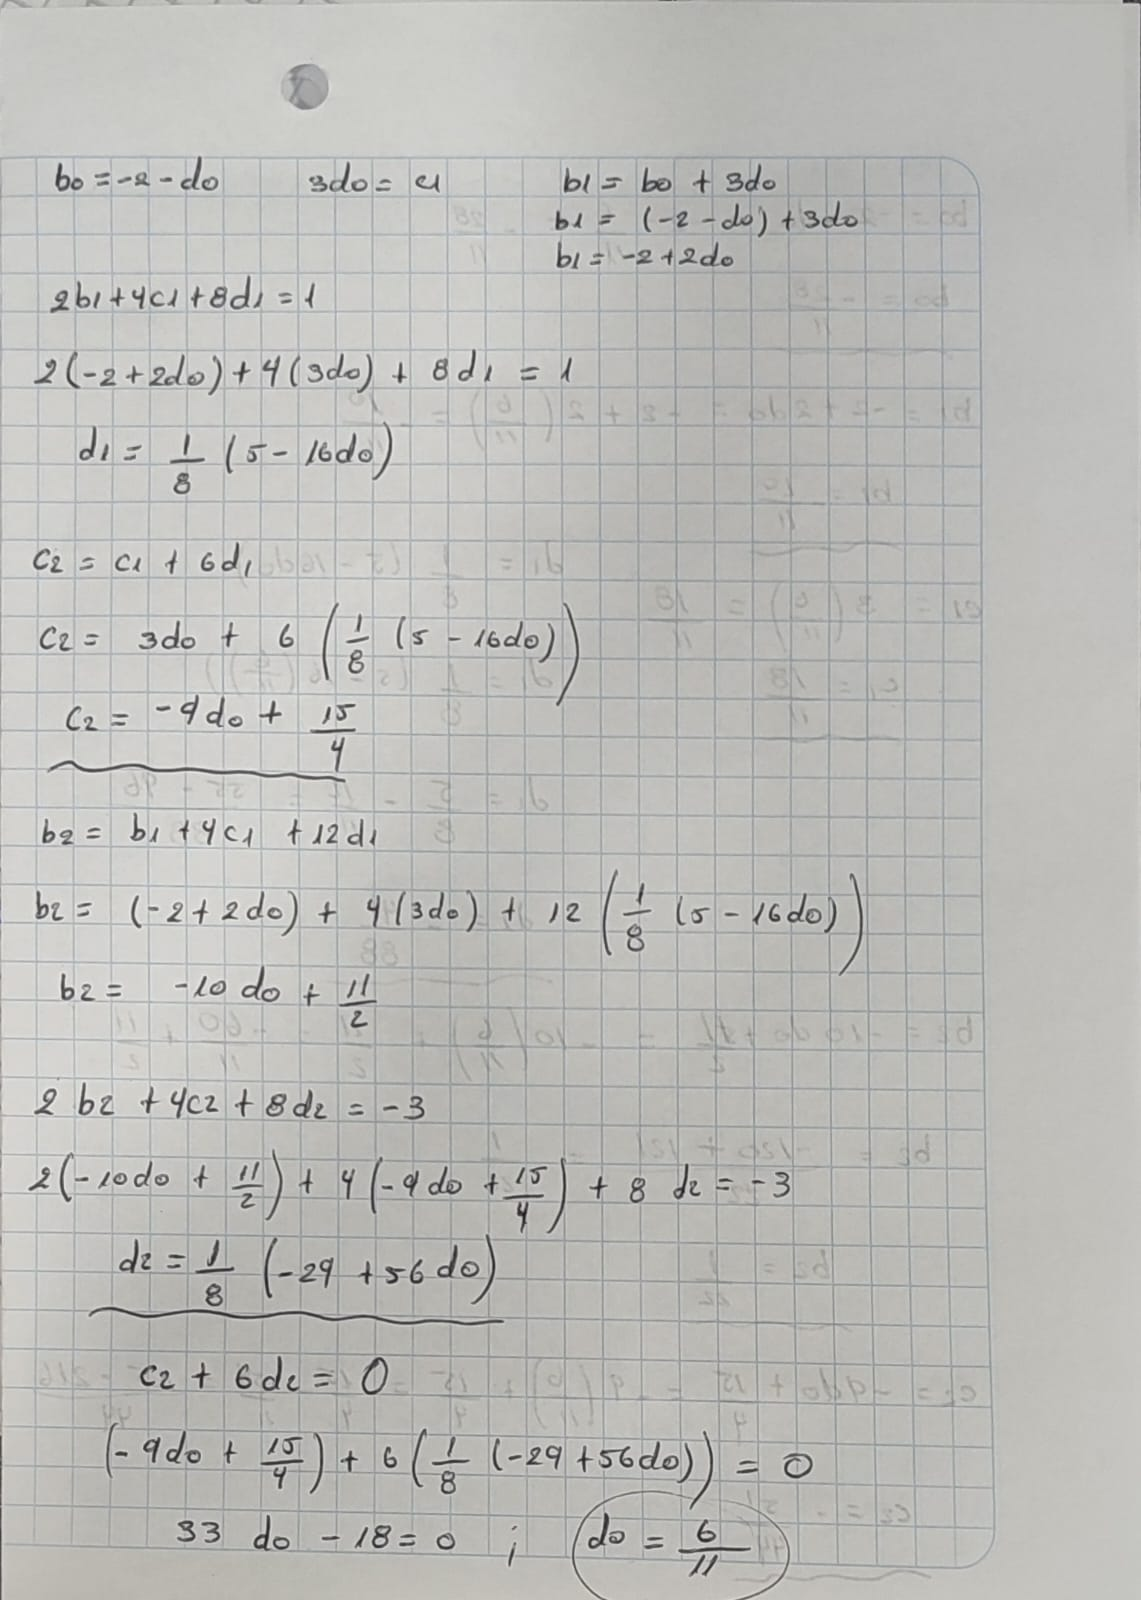
\includegraphics[width=0.5\textwidth]{inFiles/Figures/ecuacion1_1.jpeg}
        \label{fig:etiqueta}
        \end{figure}
        \begin{figure}
        \centering
        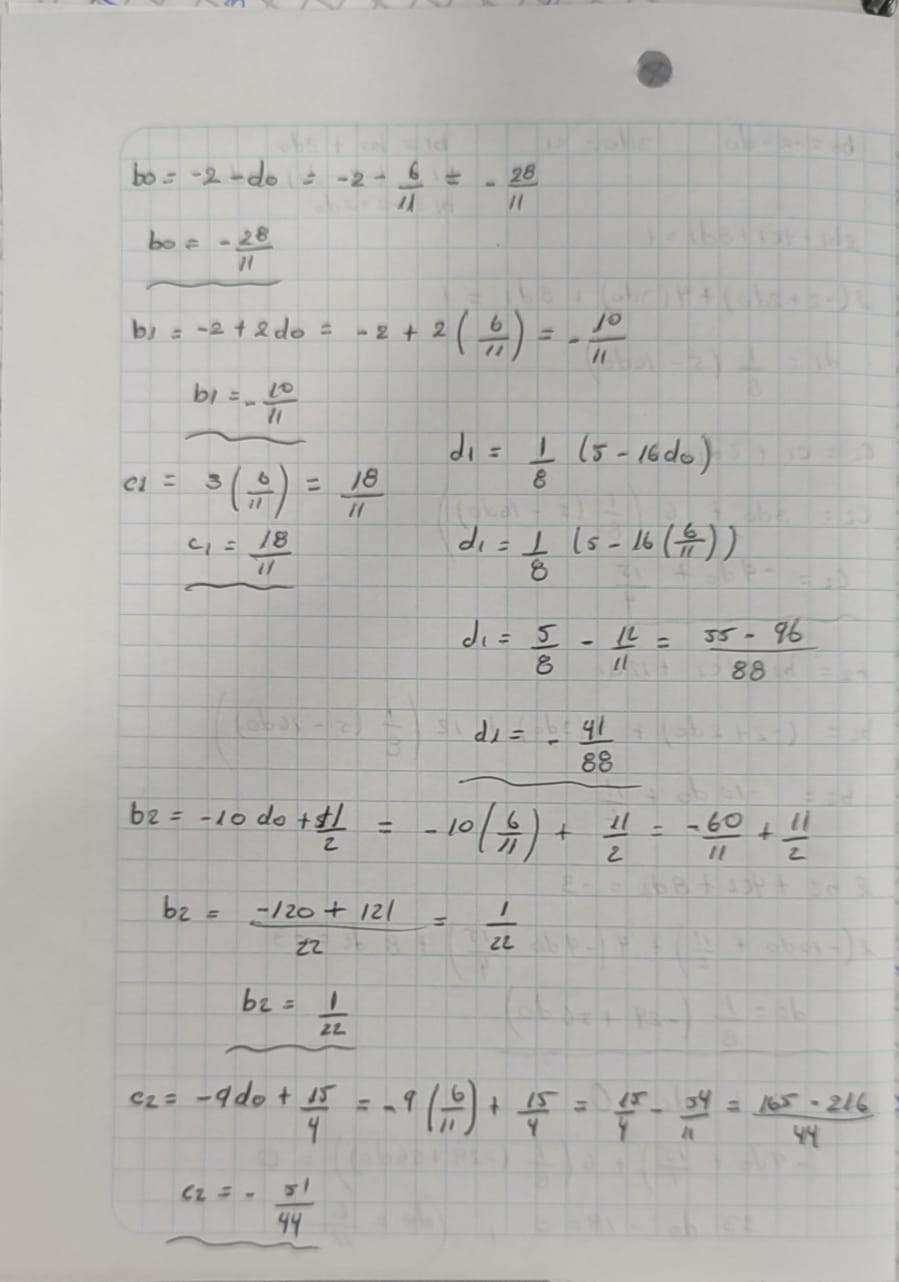
\includegraphics[width=0.5\textwidth]{inFiles/Figures/ecuacion1_2.jpeg}
        \label{fig:etiqueta}
        \end{figure}
                \begin{figure}
        \centering
        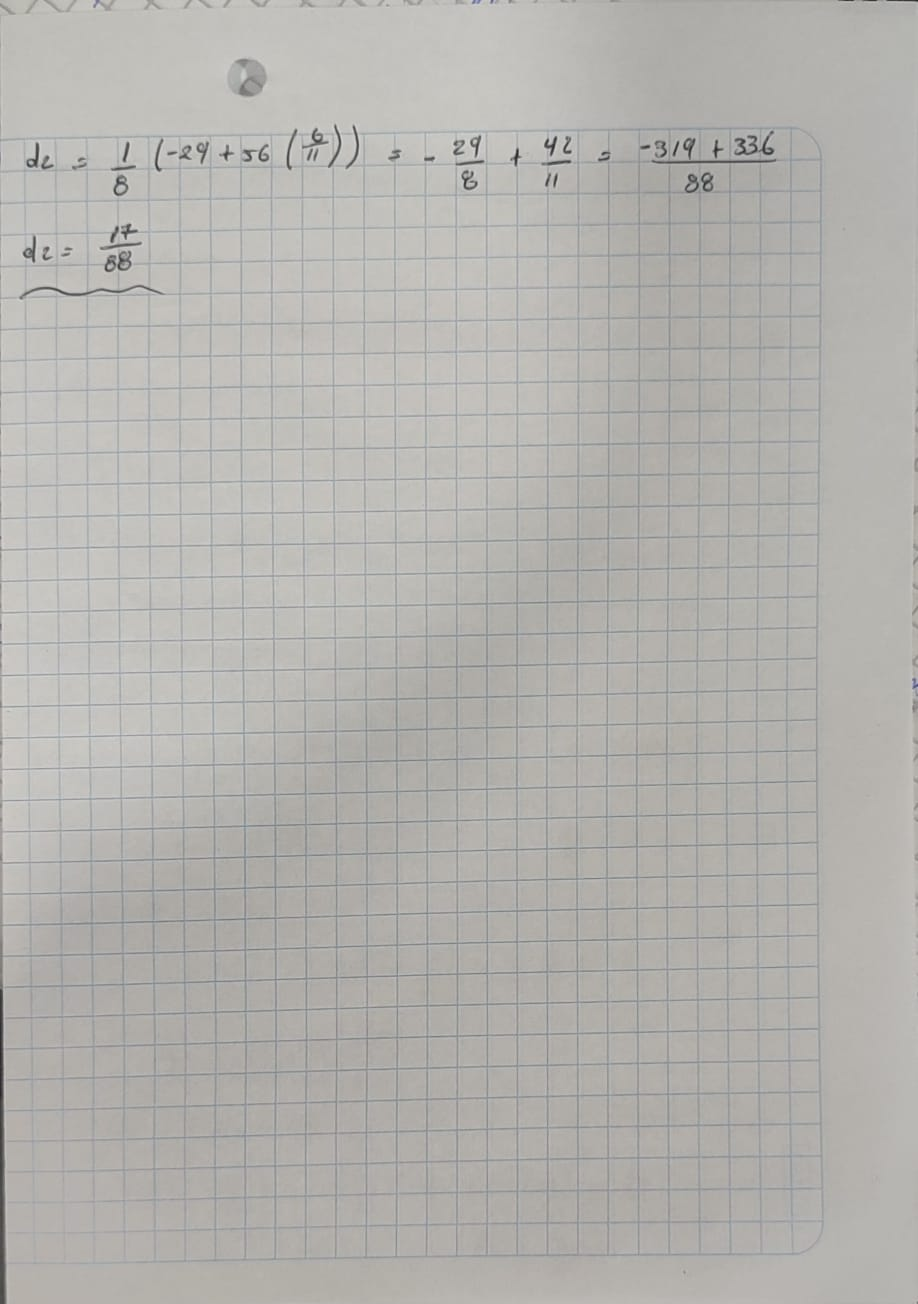
\includegraphics[width=0.5\textwidth]{inFiles/Figures/ecuacion1_3.jpeg}
        \label{fig:etiqueta}
        \end{figure}




        \
        \
        \

        Incognitas:
        \begin{table}[h]
        \centering
        \begin{tabular}{|c|c|c|c|}
        \hline
        $a_0$& 3 &$c_1$& 1.63636 \\\hline 
        $b_0$& -2.54545 &$d_1$& -0.46590 \\\hline
        $c_0$& 0 &$a_2$& 2 \\\hline
        $d_0$& 0.54545 &$b_2$& 0.04545 \\\hline
        $a_1$& 1 &$c_2$&  -1.15909\\\hline
        $b_1$& -0.90909 &$d_2$& 0.19318 \\\hline
        \end{tabular}
        \label{tab:ejemplo64}
        \end{table}
 
        
        
        \[
        \begin{aligned}
        S_0(x) &= 3 - 2.54545(x + 2) + 0.54545(x + 2)^3 \\
        S_1(x) &= 1 - 0.90909(x + 1) + 1.63636(x + 1)^2 - 0.46590(x + 1)^3 \\
        S_2(x) &= 2 + 0.04545(x - 1) - 1.15909(x - 1)^2 + 0.19318(x - 1)^3
        \end{aligned}
        \]

        
        
        
        
        
        
        
        
        
        
        
        
        
        
        
        \
        
        \item Determine el spline cúbico con frontera condicionada
        \[
        B_0 = 1 \\
        B_n = -1
        \]

        Frontera Condicionada:

        \[S'_0(x_0) = f'(x_0) = B_0\]
        \[S'_{n-1}(x_n) = f'(x_n) = B_n\]
        \begin{itemize}
            \item $S'_0(x_0) = f'(x_0) = 1$
            \[
            \begin{aligned}
            b_0 + 2c_0(x_0 - x_0) + 3d_0(x_0 - x_0)^2 &= 1\\  
            b_0 + 2c_0(0) + 3d_0(0)^2 &= 1\\  
            b_0  &= 1 \quad (11b)\\  
            \end{aligned}
            \]            
            \item $S'_2(x_3) = f'(x_3) = -1$
            \[
            \begin{aligned}
            b_2 + 2c_2(x_3 - x_2) + 3d_2(x_3 - x_2)^2 &= -1\\  
            b_2 + 2c_2(3-1) + 3d_2(3-1)^2 &= -1\\  
            b_2 + 4c_2 + 12d_2 &= -1 \quad (12b)\\  
            \end{aligned}
            \]  
        \end{itemize}
    \end{enumerate}

                Resolviendo el sistema de ecuaciones:
        \begin{figure}
        \centering
        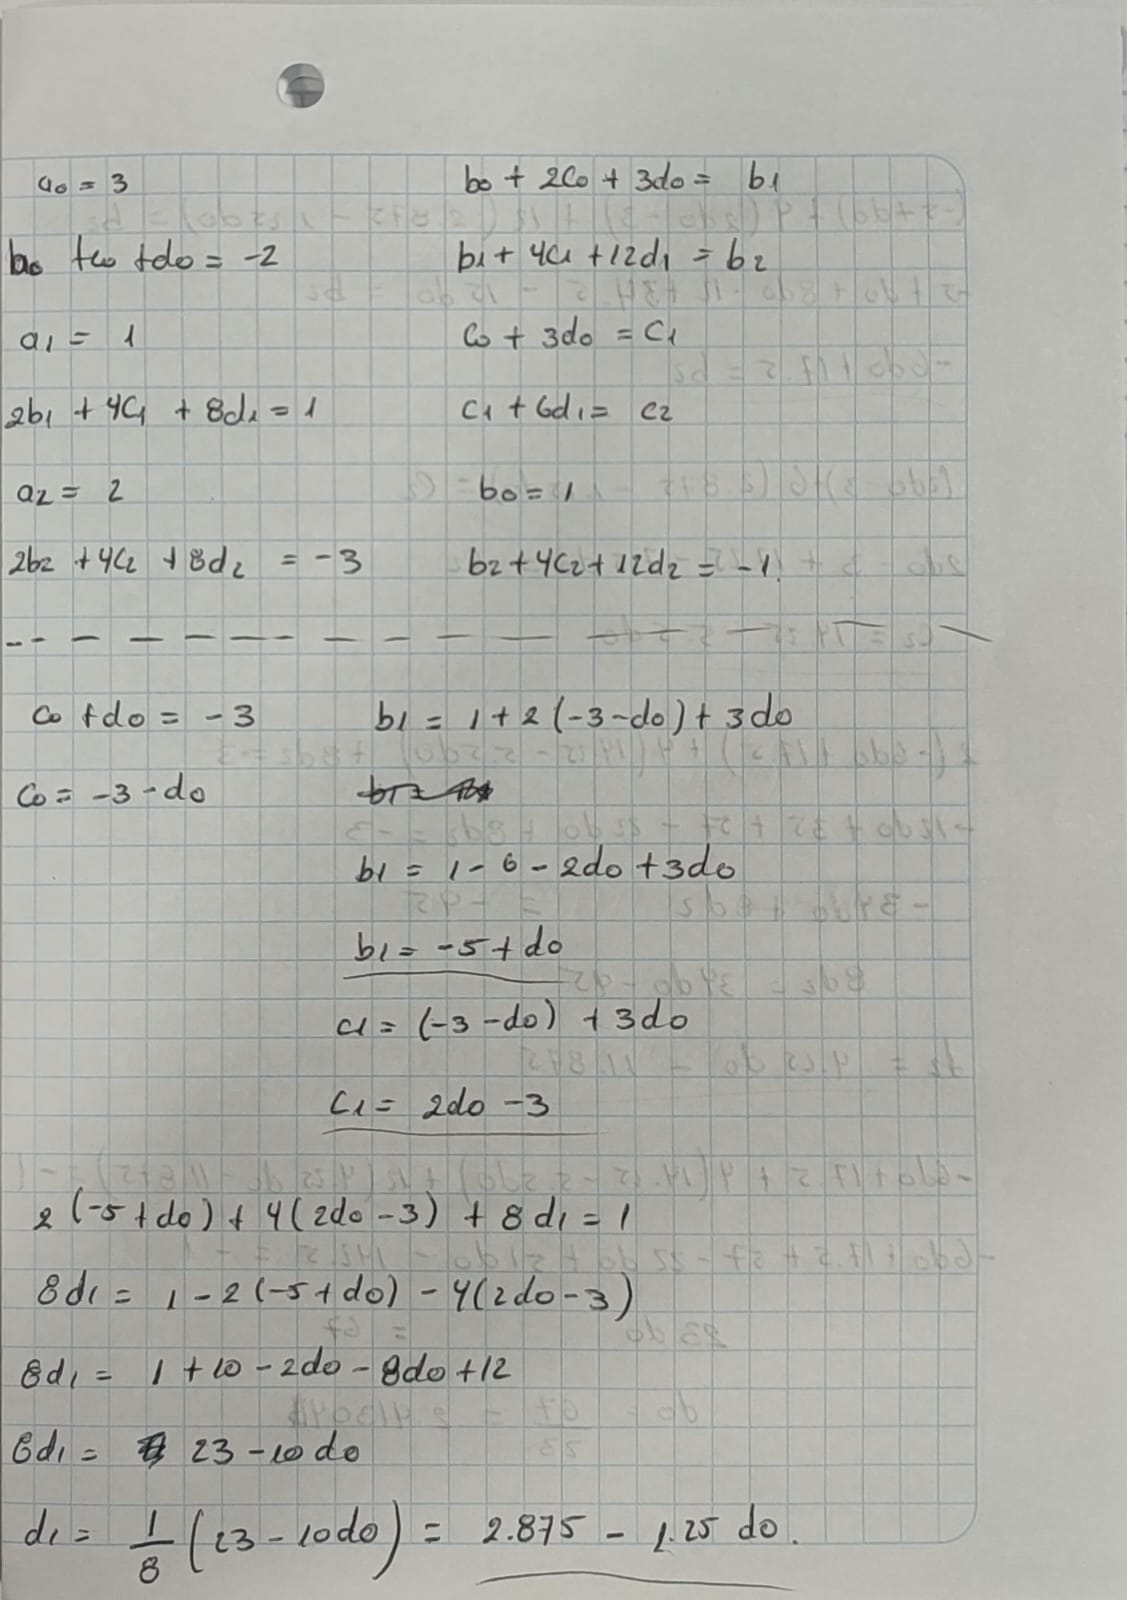
\includegraphics[width=0.5\textwidth]{inFiles/Figures/ecuacion2_1.jpeg}
        \label{fig:etiqueta}
        \end{figure}
        \begin{figure}
        \centering
        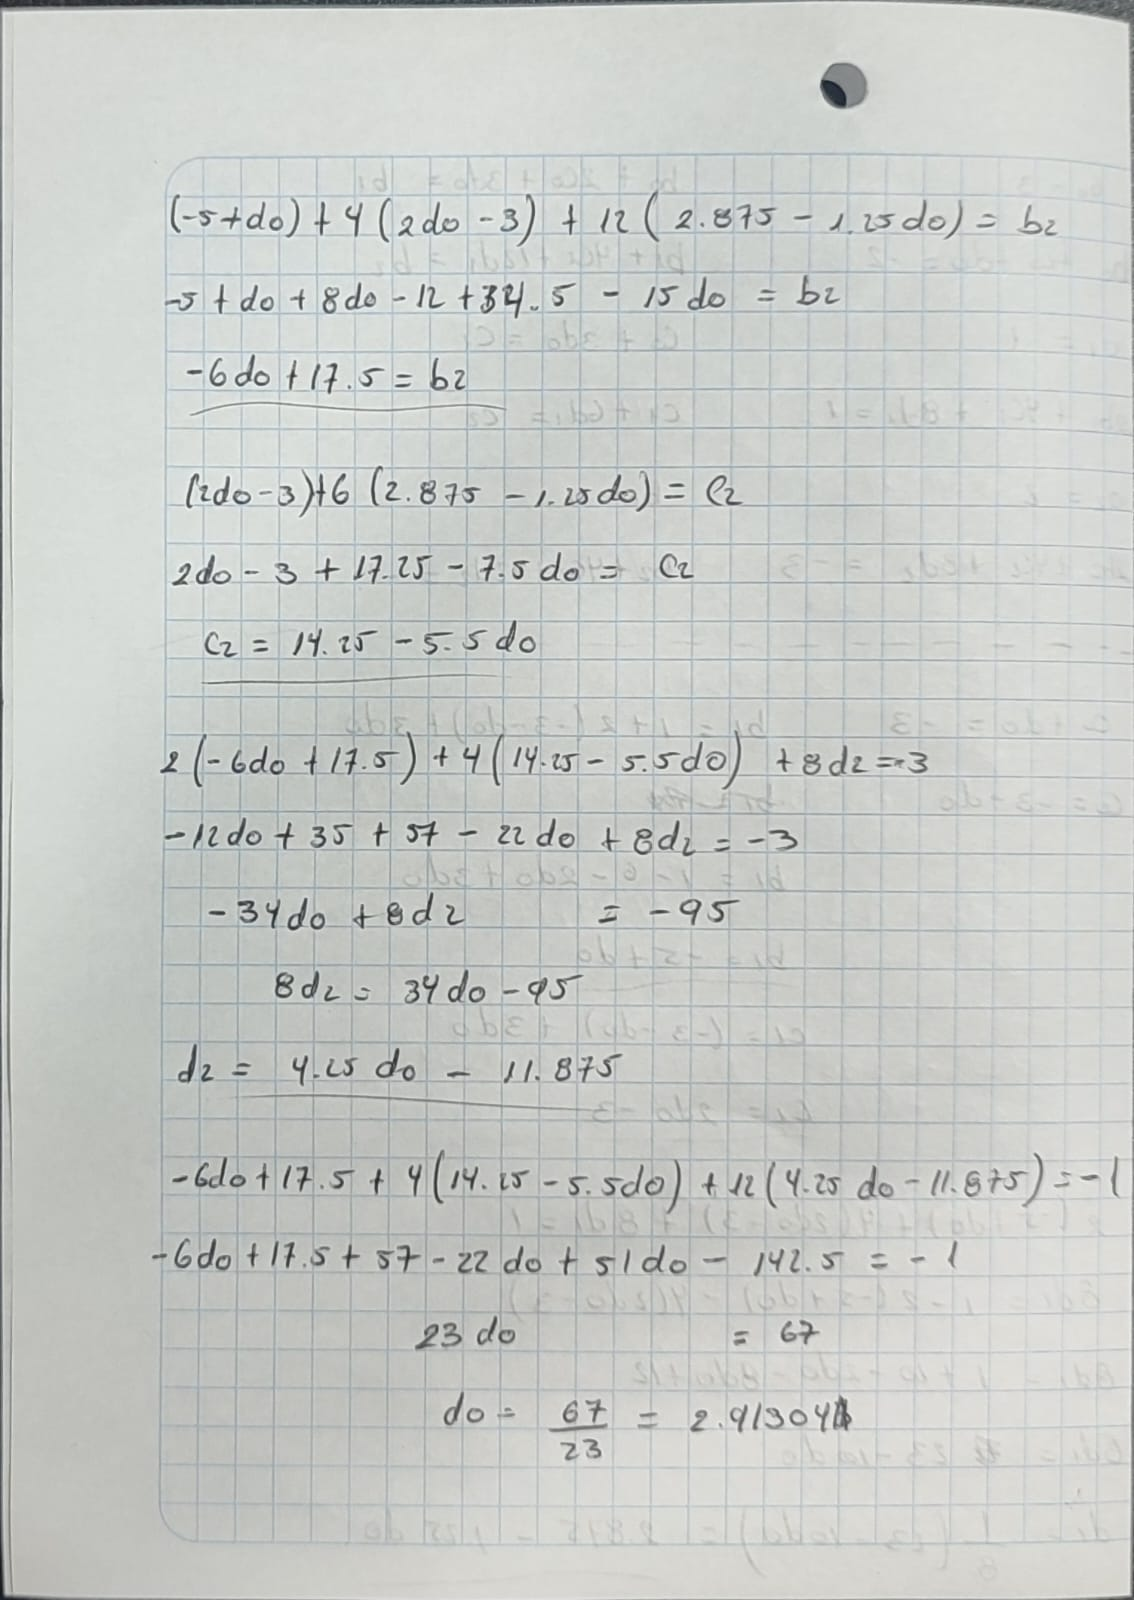
\includegraphics[width=0.5\textwidth]{inFiles/Figures/ecuacion2_2.jpeg}
        \label{fig:etiqueta}
        \end{figure}
                \begin{figure}
        \centering
        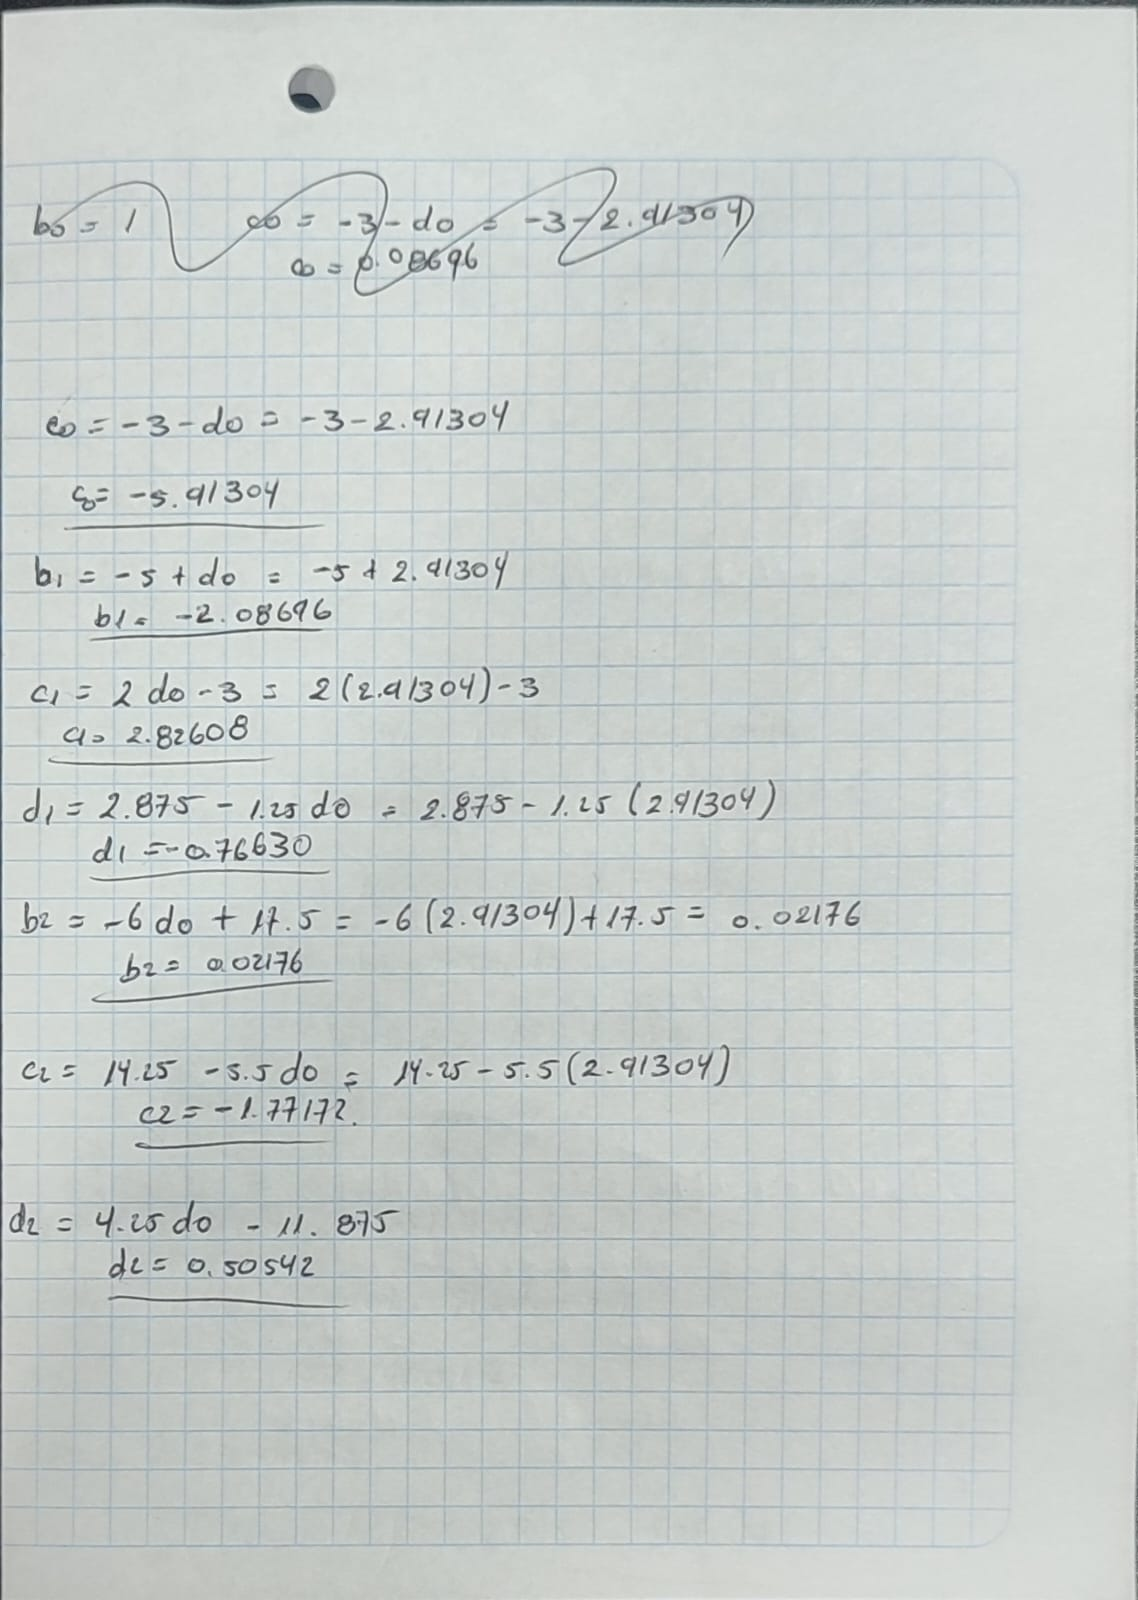
\includegraphics[width=0.5\textwidth]{inFiles/Figures/ecuacion2_3.jpeg}
        \label{fig:etiqueta}
        \end{figure}
        Incognitas:
        \begin{table}
        \centering
        \begin{tabular}{|c|c|c|c|}
        \hline
        $a_0$& 3        &$c_1$& 2.82608 \\\hline 
        $b_0$& 1        &$d_1$& -0.76630 \\\hline
        $c_0$& -5.91304 &$a_2$& 2 \\\hline
        $d_0$& 2.91304  &$b_2$& 0.02173 \\\hline
        $a_1$& 1        &$c_2$& -1.77173\\\hline
        $b_1$& -2.08695 &$d_2$& 0.50543 \\\hline
        \end{tabular}
        \end{table}

        \[
        \begin{aligned}
        S_0(x) &= 3 + 1(x + 2) - 5.91304(x + 2)^2 + 2.91304(x + 2)^3 \\
        S_1(x) &= 1 - 2.08695(x + 1) + 2.82608(x + 1)^2 - 0.76630(x + 1)^3 \\
        S_2(x) &= 2 + 0.02173(x - 1) - 1.77173(x - 1)^2 + 0.50543(x - 1)^3
        \end{aligned}
        \]

    \item Dado los puntos \( (0,1); (1,5); (2,3) \), determine el spline cúbico.
    \[x = [0 , 1, 2] \quad y = [1, 5, 3]\]
    \[ 
    \begin{aligned}
        S_0(x) &= a_0 + b_0 (x-x_0) + c_0 (x-x_0)^2 + d_0 (x-x_0)^3 = y_0 \\
        S_1(x) &= a_1 + b_1 (x-x_1) + c_1 (x-x_1)^2 + d_1 (x-x_1)^3 = y_1\\
    \end{aligned}
    \]
    
    Coincidencia con los puntos de datos.

        \begin{itemize}
            \item $S_0(x)$
            \[ 
            \begin{aligned}
                S_0(x_0) &= a_0 + b_0 (x_0-x_0) + c_0 (x_0-x_0)^2 + d_0 (x_0-x_0)^3 = y_0 \\
                S_0(x_0) &= a_0 + b_0 (0) + c_0 (0)^2 + d_0 (0)^3 = a_0 = 1 \\
                a_0 &= 1 \quad (1)\\
                S_0(x_1) &= a_0 + b_0 (x_1-x_0) + c_0 (x_1-x_0)^2 + d_0 (x_1-x_0)^3 = y_1\\
                S_0(x_1) &= 1 + b_0 (1-0) + c_0 (1-0)^2 + d_0 (1-0)^3 = 5\\
                S_0(x_1) &= b_0 + c_0 + d_0 = 4\\
                b_0& + c_0 + d_0 = 4 \quad (2)\\
            \end{aligned}
            \]
            \item $S_1(x)$
            \[ 
            \begin{aligned}
                S_1(x_1) &= a_1 + b_1 (x_1-x_1) + c_1 (x_1-x_1)^2 + d_1 (x_1-x_1)^3 = y_1 \\
                S_1(x_1) &= a_1 + b_1 (0) + c_1 (0)^2 + d_1 (0)^3 = a_1 = 5 \\
                a_1 &= 5 \quad (3)\\
                S_1(x_2) &= a_1 + b_1 (x_2-x_1) + c_1 (x_2-x_1)^2 + d_1 (x_2-x_1)^3 = y_2\\
                S_1(x_2) &= 5 + b_1 (2-1) + c_1 (2-1)^2 + d_1 (2-1)^3 = 3\\
                S_1(x_2) &=  b_1+ c_1 + d_1= -2\\
                b_1 &+ c_1 + d_1= -2 \quad (4)\\
            \end{aligned}
            \]
        \end{itemize}
    
        Continuidad de la primera derivada:
        \[S'_j(x) = b_j + 2c_j(x - x_j) + 3d_j(x - x_j)^2\]
        
        \begin{itemize}
            \item $S'_0(x_1) =  S'_1(x_1)$
            \[
            \begin{aligned}
            b_0 + 2c_0(x_1 - x_0) + 3d_0(x_1 - x_0)^2 &= b_1 + 2c_1(x_1 - x_1) + 3d_1(x_1 - x_1)^2 \\
            b_0 + 2c_0(1-0) + 3d_0(1-0)^2 &= b_1 + 2c_1(0) + 3d_1(0)^2 \\
            b_0 + 2c_0 + 3d_0 &= b_1 \quad (7) \\
            \end{aligned}
            \]
        \end{itemize}

        Continuidad de la segunda derivada:

        \[S''_j(x) = 2c_j + 6d_j(x -x_j)\]
        
        \begin{itemize}
            \item $S''_0(x_1) = S''_1(x_1)$
            \[
            \begin{aligned}
            2c_0 + 6d_0(x_1 -x_0) &= 2c_1 + 6d_1(x_1 -x_1) \\     
            2c_0 + 6d_0(1-0) &= 2c_1 + 6d_1(0) \\     
            c_0 + 3d_0 &= c_1 \quad (9) \\     
            \end{aligned}
            \]
        \end{itemize}

        por Frontera Natural:
        \[
        \begin{aligned}
        S_0''(x_0) &= S_1''(x_2) = 0 \\
        2c_0 + 6d_0(x_0 - x_0) &= 2c_1 + 6d_1(x_2 - x_1) = 0 \\
        2c_0 + 6d_0(0) &= 2c_2 + 6d_2(2 - 1) = 0 \\
        2c_0 &= 2c_1 + 6d_1(1) = 0 \\
        c_0 &= 2c_1 + 6d_1 = 0 \\
        c_0 = 0 \quad (7) &\land c_1 + 3d_1 = 0 \quad (8)\\
        \end{aligned}
        \]


        Incognitas:
        \begin{table}
        \centering
        \begin{tabular}{|c|c|}
        \hline
        $a_0$& 1    \\\hline 
        $b_0$& 5.5     \\\hline
        $c_0$& 0        \\ \hline
        $d_0$& -1.5     \\ \hline
        $a_1$& 5        \\ \hline
        $b_1$& 1   \\ \hline     
        $c_1$& -4.5 \\ \hline
        $d_1$& 1.5 \\ \hline
        \end{tabular}
        \end{table}

        \[
        \begin{aligned}
        S_0(x) &= 1 + 5{,}5\,x - 1{,}5\,x^3 \\
        S_1(x) &= 5 + 1(x - 1) - 4{,}5(x - 1)^2 + 1{,}5(x - 1)^3
        \end{aligned}
        \]  

    
    \item Dado los puntos \( (-1,1); (1,3); (0.5,4.8) \), determine el spline cúbico sabiendo que 
    \[
    f'(x_0) = 1,\quad f'(x_n) = 2.
    \]

    \[x = [-1,0.5, 1 ] \quad y = [1, 4.8,3]\]
    \[
    \begin{aligned}
        S_0(x) &= a_0 + b_0 (x-x_0) + c_0 (x-x_0)^2 + d_0 (x-x_0)^3 = y_0 \\
        S_1(x) &= a_1 + b_1 (x-x_1) + c_1 (x-x_1)^2 + d_1 (x-x_1)^3 = y_1\\
    \end{aligned}
    \]

Coincidencia con los puntos de datos.

    \begin{itemize}
        \item $S_0(x)$
        \[ 
        \begin{aligned}
            S_0(x_0) &= a_0 + b_0 (x_0-x_0) + c_0 (x_0-x_0)^2 + d_0 (x_0-x_0)^3 = y_0 \\
            S_0(x_0) &= a_0 + b_0 (0) + c_0 (0)^2 + d_0 (0)^3 = a_0 = 1 \\
            a_0 &= 1 \quad (1)\\
            S_0(x_1) &= a_0 + b_0 (x_1-x_0) + c_0 (x_1-x_0)^2 + d_0 (x_1-x_0)^3 = y_1\\
            S_0(x_1) &= 1 + b_0 (0.5 +1) + c_0 (0.5 +1)^2 + d_0 (0.5 +1)^3 = 4.8\\
            S_0(x_1) &= 1.5b_0 + 2.25c_0 + 3.375d_0 = 3.8\\
            1.5b_0& + 2.25c_0 + 3.375d_0 = 3.8 \quad (2)\\
        \end{aligned}
        \]
        \item $S_1(x)$
        \[ 
        \begin{aligned}
            S_1(x_1) &= a_1 + b_1 (x_1-x_1) + c_1 (x_1-x_1)^2 + d_1 (x_1-x_1)^3 = y_1 \\
            S_1(x_1) &= a_1 + b_1 (0) + c_1 (0)^2 + d_1 (0)^3 = a_1 = 4.8 \\
            a_1 &= 4.8 \quad (3)\\
            S_1(x_2) &= a_1 + b_1 (x_2-x_1) + c_1 (x_2-x_1)^2 + d_1 (x_2-x_1)^3 = y_2\\
            S_1(x_2) &= 4.8 + b_1 (1-0.5) + c_1 (1-0.5)^2 + d_1 (1-0.5)^3 = 3\\
            S_1(x_2) &=  0.5 b_1+ 0.25c_1 + 0.125d_1= -1.8\\
            0.5 b_1&+ 0.25c_1 + 0.125d_1= -1.8 \quad (4)\\
        \end{aligned}
        \]
    \end{itemize}

    Continuidad de la primera derivada:
        \[S'_j(x) = b_j + 2c_j(x - x_j) + 3d_j(x - x_j)^2\]
        
        \begin{itemize}
            \item $S'_0(x_1) =  S'_1(x_1)$
            \[
            \begin{aligned}
            b_0 + 2c_0(x_1 - x_0) + 3d_0(x_1 - x_0)^2 &= b_1 + 2c_1(x_1 - x_1) + 3d_1(x_1 - x_1)^2 \\
            b_0 + 2c_0(0.5+1) + 3d_0(0.5+1)^2 &= b_1 + 2c_1(0) + 3d_1(0)^2 \\
            b_0 + 3c_0 + 6.75d_0 &= b_1 \quad (5) \\
            \end{aligned}
            \]
        \end{itemize}

        Continuidad de la segunda derivada:

        \[S''_j(x) = 2c_j + 6d_j(x -x_j)\]
        
        \begin{itemize}
            \item $S''_0(x_1) = S''_1(x_1)$
            \[
            \begin{aligned}
            2c_0 + 6d_0(x_1 -x_0) &= 2c_1 + 6d_1(x_1 -x_1) \\     
            2c_0 + 6d_0(0.5+1) &= 2c_1 + 6d_1(0) \\     
            2c_0 + 9d_0 &= 2c_1 \quad (6) \\     
            \end{aligned}
            \]
        \end{itemize}

        por Frontera Condicionada:
        \begin{itemize}
            \item $S'_0(x_0) = f'(x_0) = B_0$
            \[
            \begin{aligned}
                b_0 &+ 2c_0(x_0-x_0) + 3d_0 (x_0 - x_0)^2 = 1\\
                b_0 &+ 2c_0(0) + 3d_0 (0)^2 = 1\\
                b_0 &= 1\\
            \end{aligned}
            \]
            \item $S'_1(x_2) = f'(x_2) = 2$
            \[
            \begin{aligned}
                b_2 &+ 2c_1 (x_2 - x_1) + 3d_1(x_2 - x_1)^2 = 2 \\
                b_2 &+ 2c_1 (1-0.5) + 3d_1(1-0.5)^2 = 2 \\
                b_2 &+ c_1 + 0.75d_1 = 2 \quad (8) \\
            \end{aligned}
            \]
        \end{itemize}

                Incognitas:
        \begin{table}
        \centering
        \begin{tabular}{|c|c|}
        \hline
        $a_0$& 1    \\\hline 
        $b_0$& 1     \\\hline
        $c_0$& 6.38333        \\ \hline
        $d_0$& -3.57     \\ \hline
        $a_1$& 4.8        \\ \hline
        $b_1$& -3.975 \\ \hline     
        $c_1$& -9.7 \\ \hline
        $d_1$& 20.9 \\ \hline
        \end{tabular}
        \end{table}


        \[
        \begin{aligned}
        S_0(x) &= 1 + 1(x + 1) + 6.38333(x + 1)^2 - 3.57407(x + 1)^3 \\
        S_1(x) &= 4.8 - 3.975(x - 0.5) - 9.7(x - 0.5)^2 + 20.9(x - 0.5)^3
        \end{aligned}
        \]
\end{enumerate}

%\section*{CONCLUSIONES}
%\begin{itemize}
%    \item {El polinomio de Taylor nos ayuda a aproximar funciones cuando se tenga conocimiento de las derivadas}
%    \item {El polinomio de Lagrange nos da directamente sin necesidad de derivadas} 
%\end{itemize}

%\section*{RECOMENDACIONES}

%\begin{itemize}
 %   \item Se recoienda usar la serie de Taylor siempre que se tenga conocimiento de las derivadas.
 %   \item Cuando no es posible conocer la derivada se recoimienda usar Lagrange
%\end{itemize}

%\renewcommand{\refname}{\MakeUppercase{REFERENCIAS}}
%\bibliographystyle{IEEEtran}
%\bibliography{inFiles/References/references.bib}


\end{document}
